% Тут используется класс, установленный на сервере Papeeria. На случай, если
% текст понадобится редактировать где-то в другом месте, рядом лежит файл matmex-diploma-custom.cls
% который в момент своего создания был идентичен классу, установленному на сервере.
% Для того, чтобы им воспользоваться, замените matmex-diploma на matmex-diploma-custom
% Если вы работаете исключительно в Papeeria то мы настоятельно рекомендуем пользоваться
% классом matmex-diploma, поскольку он будет автоматически обновляться по м⎄ере внесения корректив
%

% По умолчанию используется шрифт 14 размера. Если нужен 12-й шрифт, уберите опцию [14pt]
%\documentclass[14pt]{matmex-diploma}
\documentclass[14pt]{matmex-diploma-custom}

\hyphenation{op-tical net-works semi-conduc-tor con-tract Et-he-re-um}
\hyphenation{пре-по-да-ва-тель сту-дент вы-чис-ли-тель-но}
\newcommand\name[1]{\textsc{#1}}
\newcommand\achtung[1]{{\color{red}#1}}

\usepackage{amssymb,amsmath,cancel,cite,color,cmap,float,
	graphicx, multirow,pgfplots,tikz,wrapfig,xcolor,caption, 
	subcaption}

% tikz settings
\usetikzlibrary{shapes,arrows,positioning}
\tikzset{
	node distance=5cm,
	every state/.style={ 
		semithick,
		fill=gray!10
	},
	every edge/.style={
		draw,
		->,>=stealth, 
		auto,
		semithick
	}
}
\pgfplotsset{compat=1.3}

\usepackage{graphicx}
\usepackage{hyperref}
\hypersetup{
    colorlinks=true,
    linkcolor=black,
    filecolor=magenta,
    urlcolor=blue,
}
% code listings settings
\usepackage{listings}
% replace Listing in code caption
\renewcommand{\lstlistingname}{Листинг}
\usepackage{xcolor}

\definecolor{codegreen}{rgb}{0,0.6,0}
\definecolor{codegray}{rgb}{0.5,0.5,0.5}
\definecolor{codepurple}{rgb}{0.58,0,0.82}
\definecolor{backcolour}{rgb}{0.95,0.95,0.92}

\lstdefinestyle{mystyle}{
    backgroundcolor=\color{backcolour},   
    commentstyle=\color{codegreen},
    keywordstyle=\color{magenta},
    numberstyle=\tiny\color{codegray},
    stringstyle=\color{codepurple},
    basicstyle=\ttfamily\footnotesize,
    breakatwhitespace=false,         
    breaklines=true,                 
    captionpos=b,                    
    keepspaces=true,                 
    numbers=left,                    
    numbersep=5pt,                  
    showspaces=false,                
    showstringspaces=false,
    showtabs=false,                  
    tabsize=2
}

\lstdefinelanguage{my_pseudo} {
	morekeywords={function, for, return, let, in},
	sensitive=false,
	morecomment=[l]{//},
	morecomment=[s]{/*}{*/},
	morestring=[b]",
}

\lstset{style=mystyle}
\lstset{language=my_pseudo}

\begin{document}
%% Если что-то забыли, при компиляции будут ошибки Undefined control sequence \my@title@<что забыли>@ru
%% Если англоязычная титульная страница не нужна, то ее можно просто удалить.
\filltitle{ru}{
    %% Актуально только для курсовых/практик. ВКР защищаются не на кафедре а в ГЭК по направлению, 
    %%   и к моменту защиты вы будете уже не в группе.
%    chair              = {},
%    group              = {},
    %% Макрос filltitle ненавидит пустые строки, поэтому обязателен хотя бы символ комментария на строке
    %% Актуально всем.
    title              = {Исследование применимости специализации алгоритма Витерби скрытой марковской моделью},
    % 
    %% Здесь указывается тип работы. Возможные значения:
    %%   coursework - отчёт по курсовой работе;
    %%   practice - отчёт по учебной практике;
    %%   prediploma - отчёт по преддипломной практике;
    %%   master - ВКР магистра;
    %%   bachelor - ВКР бакалавра.
    type               = {master},
    author             = {Тюляндин Иван Владимирович},
    % 
    %% Актуально только для ВКР. Указывается код и название направления подготовки. Типичные примеры:
    %%   02.03.03 <<Математическое обеспечение и администрирование информационных систем>>
    %%   02.04.03 <<Математическое обеспечение и администрирование информационных систем>>
    %%   09.03.04 <<Программная инженерия>>
    %%   09.04.04 <<Программная инженерия>>
    %% Те, что с 03 в середине --- бакалавриат, с 04 --- магистратура.
    specialty          = {09.04.04 <<Программная инженерия>>},
    % 
    %% Актуально только для ВКР. Указывается шифр и название образовательной программы. Типичные примеры:
    %%   СВ.5006.2017 <<Математическое обеспечение и администрирование информационных систем>>
    %%   СВ.5162.2020 <<Технологии программирования>>
    %%   СВ.5080.2017 <<Программная инженерия>>
    %%   ВМ.5665.2019 <<Математическое обеспечение и администрирование информационных систем>>
    %%   ВМ.5666.2019 <<Программная инженерия>>
    %% Шифр и название программы можно посмотреть в учебном плане, по которому вы учитесь. 
    %% СВ.* --- бакалавриат, ВМ.* --- магистратура. В конце --- год поступления (не обязательно ваш, если вы были в академе/вылетали).
    programme          = {ВМ.5666.2019 <<Программная инженерия>>},
    % 
    %% Актуально только для ВКР, только для матобеса и только 2017-2018 годов поступления. Указывается профиль подготовки, на котором вы учитесь.
    %% Названия профилей можно найти в учебном плане в списке дисциплин по выбору. На каком именно вы, вам должны были сказать после второго курса (можно уточнить в студотделе).
    %% Вот возможные вариканты:
    %%   Математические основы информатики
    %%   Информационные системы и базы данных
    %%   Параллельное программирование
    %%   Системное программирование
    %%   Технология программирования
    %%   Администрирование информационных систем
    %%   Реинжиниринг программного обеспечения
    % profile            = {Системное программирование},
    % 
    %% Актуально всем.
    %supervisorPosition = {проф. каф. СП, д.ф.-м.н., проф.}, % Терехов А.Н.
    supervisorPosition = {к.ф.-м.н., доцент кафедры информатики\\}, % Григорьев С.В.   
    supervisor         = {С. В. Григорьев},  
    % 
    %% Актуально только для практик и курсовых. Если консультанта нет, закомментировать или удалить вовсе.
    consultantPosition = {к.ф.-м.н., старший преподаватель кафедры МКН СПбГУ\\},
    consultant         = {Д. А. Березун},
    %
    %% Актуально только для ВКР.
    reviewerPosition   = {старший преподаватель, Санкт-Петербургский Политехнический Университет\\},
    reviewer           = {М. Х. Ахин},
}

\filltitle{en}{
%     chair              = {Advisor's chair},
%     group              = {ХХB.ХХ-mm},
     title              = {Viterbi algorithm specialization with hidden Markov model},
     type               = {master},
     author             = {Ivan Tyulyandin},
%     % 
%     %% Possible choices:
%     %%   02.03.03 <<Software and Administration of Information Systems>>
%     %%   02.04.03 <<Software and Administration of Information Systems>>
%     %%   09.03.04 <<Software Engineering>>
%     %%   09.04.04 <<Software Engineering>>
%     %% Те, что с 03 в середине --- бакалавриат, с 04 --- магистратура.
     specialty          = {09.04.04 <<Software Engineering>>},
%     % 
%     %% Possible choices:
%     %%   СВ.5006.2017 <<Software and Administration of Information Systems>>
%     %%   СВ.5162.2020 <<Programming Technologies>>
%     %%   СВ.5080.2017 <<Software Engineering>>
%     %%   ВМ.5665.2019 <<Software and Administration of Information Systems>>
%     %%   ВМ.5666.2019 <<Software Engineering>>
     programme          = {ВМ.5666.2019 <<Software Engineering>>},
%     % 
%     %% Possible choices:
%     %%   Mathematical Foundations of Informatics
%     %%   Information Systems and Databases
%     %%   Parallel Programming
%     %%   System Programming
%     %%   Programming Technology
%     %%   Information Systems Administration
%     %%   Software Reengineering
%	profile            = {Software Engineering},
%     % 
%     %% Note that common title translations are:
%     %%   кандидат наук --- C.Sc. (NOT Ph.D.)
%     %%   доктор ... наук --- Sc.D.
%     %%   доцент --- docent (NOT assistant/associate prof.)
%     %%   профессор --- prof.
	supervisorPosition = {C.Sc., docent\\},
	supervisor         = {S. V. Grigorev},
%     % 
    consultantPosition = {senior lecturer at Department of Mathematics and Computer Science of SbPU, C.Sc.\\},
    consultant         = {D. A. Berezun},
%     %
     reviewerPosition   = {senior lecturer at Peter the Great St.Petersburg Polytechnic University\\},
     reviewer           = {M. H. Akhin},
}
\maketitle
\tableofcontents
% У введения нет номера главы

\section*{Введение}

Количество доступной информации в современном мире стремительно растет.
С целью повышения скорости обработки информации используются различные подходы, такие как вычислительные кластеры, новые алгоритмы и дополнительное оборудование, например, FPGA (ПЛИС) или GPGPU (графический процессор общего назначения). 
Однако на практике не всегда есть возможность увеличить имеющиеся вычислительные мощности, и в таком случае необходимо искать способы улучшения алгоритмов.

Одним из таких способов является описание и реализация отдельных шагов существующих алгоритмов  с использованием иных понятий и формализмов.
Для многих алгоритмов отдельные шаги могут быть описаны с использованием методов линейной алгебры, например, через операции над матрицами с переопределёнными операциями поэлементного сложения и умножения.
Если описать алгоритм методами линейной алгебры и запрограммировать его с использованием промышленных библиотек, то он может значительно превзойти по скорости исходную реализацию за счет возможности эффективно распараллеливания матричных операций.
Алгоритмы, которые выражены через операции и понятия из линейной алгебры, широко используются в различных областях, таких как машинное обучение~\cite{LA_ML}, компьютерное зрение~\cite{LA_CV}, статистика~\cite{LA_STAT}, анализ программ на логических языках программирования ~\cite{part_eval_logic}, теория графов~\cite{SuiteSparse} и многих других.

Другой способ улучшения алгоритмов основан на следующем наблюдении. 
Достаточно часто случается ситуация, когда часть параметров алгоритма не меняется от запуска к запуску, т.е. они зафиксированы в течение некоторого значительного промежутка времени.
Зная фактические значения этих параметров, можно оптимизировать их использование в алгоритме. 
Таким образом, можно получить новый алгоритм, в котором вычисления, зависящие только от зафиксированных параметров, уже выполнены.
Результат выполнения нового алгоритма с оставшимися параметрами должен быть семантически эквивалентен результату выполнения исходного алгоритма на соответствующих данных. 
В сравнении с исходным алгоритмом, при повторных запусках новый алгоритм не выполняет те вычисления, которые зависят от зафиксированных параметров. 
Эти вычисления сделаны и сохранены на стадии генерации нового алгоритма.
Такая техника преобразования алгоритмов известна как “специализация”, или “частичное вычисление”, а программа, генерирующая новый алгоритм, называется “специализатор”~\cite{Jones_spec}.
На текущий момент вопрос о границах применимости специализации к алгоритмам, выраженных с помощью методов линейной алгебры, до конца не исследован.

В данной работе будет рассмотрена специализация известного алгоритма Витерби~\cite{Viterbi}, выраженного в терминах линейной алгебры~\cite{LA_Viterbi}. 
Этот алгоритм используется в биоинформатике~\cite{cudampf}, при распознавании речи~\cite{Rabiner_VA} и в финансовых расчетах~\cite{Viterbi_credit}. 
У него имеется два входных параметра: скрытая марковская модель (далее --- СММ)~\cite{Eddy_HMM} и последовательность наблюдений. 
Задачей алгоритма Витерби является вычислить  вероятность того, что последовательность наблюдений была сгенерирована именно с помощью данной СММ. 
Основная часть алгоритма Витерби существенно зависит от СММ, и в то же время на практике, как правило, используется какая-то одна марковская модель для анализа значительного количества последовательностей наблюдений. 
Следовательно, если  специализировать алгоритм Витерби скрытой марковской моделью, то это может дать значительный прирост производительности.
\section{Постановка задачи}
Цель данной работы --- исследовать применимость специализации
алгоритма Витерби скрытой марковской моделью.
Если специализированная версия окажется производительнее, 
то это может ускорить исследования, проводимые биологами по 
изучению функциональности протеинов.

Были поставлены следующие задачи:
\begin{itemize}
	\item сделать обзор предметной области и существующих решений задачи 
		гомологичности;
	\item реализовать неспециализированный алгоритм Витерби;
	\item написать специализатор алгоритма Витерби на СММ;
	\item провести сравнительный анализ специализированной программы с
		неспециализированной версией и существующими решениями.
\end{itemize}

\section{Обзор}
В главе выполнен обзор предметной области.
Описаны скрытые марковские модели и алгоритм Витерби,
а также приведены существующие решения, в которых этот 
алгоритм реализован для обработки большого объёма данных.
В заключительном разделе обзора рассмотрена техника специализации.

\subsection{Скрытые марковские модели}
\label{lab:HMM}
\emph{Скрытая марковская модель} (СММ)~\cite{Eddy_HMM}
является дискретным вероятностным автоматом, каждое состояние которого может с определённой вероятностью создавать наблюдение.
В определении СММ есть следующие параметры:
\begin{itemize}
	\item $\mathit{S_{1..N}}$ --- $N$ состояний автомата;
	\item $\mathit{O_{1..K}}$ --- $K$ возможных наблюдений;
	\item $\mathit{B_{1..N}}$ --- вероятности для каждого состояния из $\mathit{S_{1..N}}$ быть стартовым;
	\item $\mathit{T_{1..N, 1..N}}$ --- матрица переходов, $\mathit{T_{i,j}}$ является вероятностью перехода из состояния
$\mathit{S_{i}}$ в состояние $\mathit{S_{j}}$;
	\item $\mathit{E_{1..N, 1..K}}$ --- матрица наблюдений, 
где $\mathit{E_{i,j}}$ определяет вероятность создания наблюдения $\mathit{O_{j}}$ в состоянии $\mathit{S_{i}}$.
\end{itemize}
Пример скрытой марковской модели представлен на рисунке~\ref{fig:HMM}.
В ней два состояния H и L, и четыре возможных наблюдения A, C, T и G.
Вероятности переходов между состояниями указаны на соответствующих стрелках, а вероятности создания определённого наблюдения описаны в состояниях.

\begin{figure}
\centering
	\begin{subfigure}{\textwidth}
		\centering
		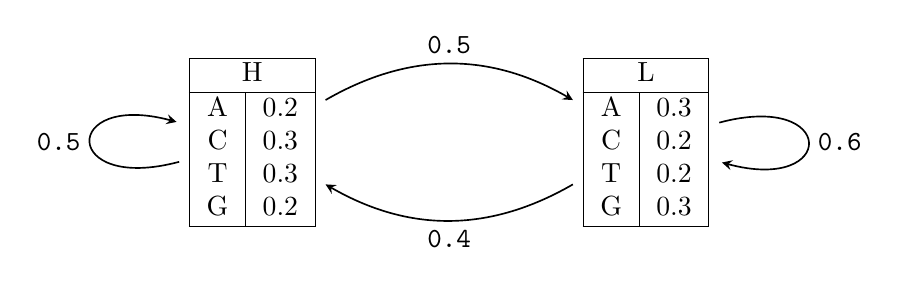
\begin{tikzpicture}
			\node (H) {
				\begin{tabular}{|c|c|}
					\hline
					\multicolumn{2}{|c|} H \\
					\hline
					A & 0.2 \\
					C & 0.3 \\
					T & 0.3 \\
					G & 0.2 \\
					\hline
				\end{tabular}
			};
			\node[right of=H] (L) {
				\begin{tabular}{|c|c|}
					\hline
					\multicolumn{2}{|c|} L \\
					\hline
					A & 0.3 \\
					C & 0.2 \\
					T & 0.2 \\
					G & 0.3 \\
					\hline
				\end{tabular}
			};
			\draw (H) edge[loop left] node {\tt 0.5} (H);
			\draw (H) edge[bend left] node {\tt 0.5} (L);
			\draw (L) edge[loop right] node {\tt 0.6} (L);
			\draw (L) edge[bend left] node {\tt 0.4} (H);
		\end{tikzpicture}
	\end{subfigure}
	\newline
	\vspace{1cm}
	\begin{subfigure}{\textwidth}
		\centering
		\begin{tabular}{c}
			Стартовые вероятности (B) \\
			\begin{tabular}{|c|c|}
				\hline
				H & L \\
				\hline
				0.5 & 0.5 \\
				\hline
			\end{tabular} \\
		\end{tabular}
		\vspace{0.3cm}
	\end{subfigure}
\caption{Пример СММ}
\label{fig:HMM}
\end{figure}


\subsection{Алгоритм Витерби}
\label{lab:Viterbi}
\emph{Алгоритм Витерби}~\cite{Viterbi} вычисляет максимальную вероятность нахождения в каждом состоянии СММ (англ. HMM) при условии того, что последовательность событий \emph{Obs} была сгенерирована этой СММ.

\subsubsection{Описание методами динамического программирования}
\label{lab:dyn_Viterbi}
Алгоритм Витерби может быть описан методами динамического программирования.
Псевдокод алгоритма представлен на листинге~\ref{lab:dyn_Viterbi}.
Массивы индексируются с единицы до границы включительно.
На строках 5-6 происходит обработка первого наблюдения из последовательности $Obs$.
Так как это первое наблюдение, то вероятности перехода учитывать не нужно.
Вычисления, связанные с оставшейся частью последовательности, выполняются на строках 8-11.
Результатом является последняя строка матрицы $Dp$.
\begin{lstlisting}[caption=Алгоритм Витерби, label=Viterbi, escapeinside={(*}{*)}]
function Viterbi(HMM, Obs)
	lo = length(Obs)
	Dp[lo][HMM.N]

	for j = 1..HMM.N
		Dp[1][j] = HMM.E[j][Obs[1]] * HMM.B[j]
	
	for i = 2..lo
		for j = 1..N
			Dp[i][j] = 
					(*$\max_{x = 1..N}$*)(HMM.T[x][j] * HMM.E[j][Obs[i]] * Dp[i-1][x])

	return Dp[lo]
\end{lstlisting}


\subsubsection{Описание методами линейной алгебры}
\label{lab:LA_Viterbi}
Также алгоритм Витерби может быть выражен матричными 
операциями из линейной алгебры~\cite{LA_Viterbi}.
Рассмотрим подробнее, как это делается.

Ключевой идеей является использование специальной 
алгебраической структуры полукольцо \emph{Min-plus}.
Элементы полукольца будут описывать вероятности с
помощью дробных чисел.
Операция сложения определяется как функция
минимума из двух чисел, а операция умножения имеет семантику
сложения чисел.
Нейтральными элементами по сложению будет $+\infty$ 
и 0 по умножению соответственно.
Ниже приведен пример умножения матрицы на столбец 
с использованием полукольца \emph{Min-plus}.
\[
  \begin{pmatrix}
    0 & 1 \\
    +\infty & 2
  \end{pmatrix}
  \begin{pmatrix}
    3 \\
    4
  \end{pmatrix}
  =
  \begin{pmatrix}
    min(0 + 3, 1 + 4) \\
    min(+\infty + 3, 2 + 4)
  \end{pmatrix}
  =
  \begin{pmatrix}
    3 \\
    6
  \end{pmatrix}
\]

Для того, чтобы можно было использовать полукольцо \emph{Min-plus}, 
ко всем вероятностям $p$ в СММ применяется 
преобразование~\ref{eq:t}.
Это делается для сохранения точности расчетов.
Далее такая вероятность будет называться \emph{преобразованной}.
Например, преобразованная вероятность 0.5
равна $-1 * log_2(0.5) = 1$.
\begin{equation}
t(p) =
	\begin{cases}
	p > 0: & -1 * log_{2}(p))\\
	p = 0: & +\infty
	\end{cases}       
  \label{eq:t}
\end{equation}

Для каждого события \emph{o} из множества \emph{O} 
определяем диагональную матрицу $P(o)$ размера $N \times N$.
\[
  P(o) =
  \begin{pmatrix}
    t(E[1,o]) & \hdots & +\infty \\
    \vdots & \ddots & \vdots\\
    +\infty & \hdots & t(E[N,o])
  \end{pmatrix}
\]

Начало алгоритма Витерби --- это обработка первого наблюдения 
из последовательности \emph{Obs}.
В столбце \emph{B} хранятся преобразованные вероятности 
состояний из СММ быть начальными.
Символ $\times$ обозначает умножение матриц с использованием 
полукольца \emph{Min-plus}.
\[Probs_{1} = P(Obs[1]) \times B\]
Далее вычисляются преобразованные вероятности для всех 
состояний СММ с учётом ос\-тавшихся событий из \emph{Obs}.
Матрица \emph{T} хранит преобразованные вероятности 
переходов из состояния в состояние.
В отличие от обработки первого наблюдения, далее необходимо 
учитывать и вероятности перехода, и вероятности создания 
наблюдения.
Обработка происходит следующим образом:
\[Probs_{t} = P(Obs[t]) \times T^{\top} \times Probs_{t - 1}\]
После выполнения всех шагов алгоритма, в столбце 
\emph{Probs\textsubscript{lo}}, где $lo$ --- это длина 
последовательности $Obs$, будут находиться преобразованные 
вероятности быть в определённом состоянии СММ при условии 
наблюдения последовательности событий \emph{Obs}.
Псевдокод алгоритма приведен на листинге~\ref{LA_Viterbi}.
\begin{lstlisting}[caption={Алгоритм Витерби, выраженный методами линейной алгебры}, label=LA_Viterbi, escapeinside={(*}{*)}]
function Viterbi(HMM, Obs)
	lo = length(Obs)
	// (*\textcolor{codegreen}{Столбец для результатов}*)
	Probs[1][HMM.N]

	// (*\textcolor{codegreen}{Все матричные умножения выполняются в полукольце Min-plus}*)
	Probs = P(Obs[1]) (*$\times$*) HMM.B
	
	for i = 2..lo
		Probs = P(Obs[i]) (*$\times$*) (HMM.T)(*$^{\top}$*) (*$\times$*) Probs
		
	return Probs
\end{lstlisting}


\subsection{Существующие реализации алгоритма Витерби}
\label{lab:exist_Viterbi}
В данном разделе рассмотрены существующие 
высокопроизводительные реализации алгоритма Витерби, которые 
используются на практике в бионформатике для решения задачи 
гомологичности, то есть для определения схожести протеинов.
Группы схожих протеинов называются \emph{семейством},
на основе которого можно построить СММ, описывающую общие 
части протеинов из семейства.
Такая СММ называется \emph{профилем}.
Все протеины кодируются двадцатью аминокислотами, 
которые могут быть выражены буквами латинского алфавита.
Последовательность, обрабатываемая с помощью профиля, также 
является закодированным протеином.

Рассмотренные далее реализации алгоритма Витерби выполнены с 
использованием метода динамического программирования.
Этот метод описан в подразделе~\ref{lab:dyn_Viterbi}.

\subsubsection{\name{HMMer}}
\label{lab:HMMer}
Решение \name{HMMer}~\cite{HMMer} используется для поиска в базах 
данных последовательностей гомологов исследуемых протеинов, а 
также для создания профилей семейств протеинов.
Этот проект является открытым (open source project), реализован  на языке C с возможностью
использовать SIMD-инструкции процессора.
Успешно применяется во многих базах данных, таких как \name{Pfam}~\cite{Pfam}.

Авторами проекта были предложены вероятностные \emph{фильтры}.
Их применение позволяет ускорить обработку данных из-за 
уменьшения вычислений в алгоритме Витерби за счет уменьшения 
количества состояний и переходов в СММ.
Один из таких фильтров --- \name{MSV} (Multiple Segment 
Viterbi)~\cite{MSV_Eddy}.

\subsubsection{\name{CUDAMPF}}
\label{lab:CUDAMPF}
В проекте \name{CUDAMPF}~\cite{cudampf} реализованы
вероятностные фильтры из существующего решения \name{HMMer} с использованием 
\name{CUDA}.
Код предназначен для видеокарт \name{NVIDIA} с 
архитектурой \name{Kepler} или более новой.
Проект рассчитан на определение гомологичности одновременно 
для множества протеинов.

Авторы предлагают четыре уровня параллелизма.
Первые три основаны на логическом параллелизме по данным.
Четвертый уровень использует \name{SIMD}-инструкции 
вычислителей видеокарты.
Разделение данных по уровням позволило добиться ускорения в 
23,1 раз при работе с фильтром \name{MSV} по сравнению с
\name{HMMer}.

Несмотря на то, что авторами заявлена корректность 
реализации, в исходном коде есть гонка данных при вычислении 
одного из состояний при обработке \name{MSV}.
В этом состоянии хранится максимум из определённого множества состояний.
В коде \name{CUDAMPF} переменная, хранящая максимум, 
не защищена от одновременной записи двумя или более потоками.

\subsection{Специализация}
Техника \emph{специализации} (или \emph{частичных вычислений}) предназначена для
преобразования программ, у которых часть входных параметров
известна и зафиксирована~\cite{Jones_spec} с целью оптимизации производительности.
Типичным случаем для специализации является последовательное 
применение программы для обработки данных, часть из которых 
не меняется от запуска к запуску.
Согласно определениям, которые приняты для специализации, 
зафиксированные параметры называются \emph{статическими}, а 
все остальные параметры --- \emph{динамическими}.
Цель применения специализации --- уменьшить количество 
вычислений, которые зависят от статических параметров.
Ожидается, что при многочисленных запусках специализированная 
программа на динамических параметрах будет более 
производительной чем изначальная версия программы, которая 
выполняется на статических и динамических параметрах.
Распространённой проблемой на практике является замедление 
производительности из-за большого объема специализированного
кода.
Схема специализации приведена на рисунке~\ref{spec}.
\begin{figure}[h!]
  \centering
  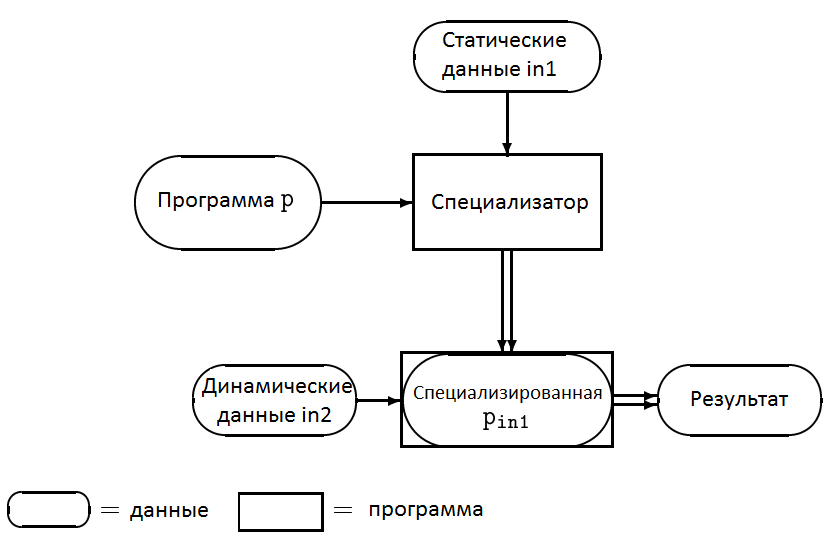
\includegraphics[width=\columnwidth]{spec.png}
  \caption{Концептуальная схема специализации~\cite{Jones_spec}}
  \label{spec}
\end{figure}

Специализация была успешно применена в обработке 
графики~\cite{RT_spec}, обработке запросов к базам 
данных~\cite{SQL_spec} и поиску подстроки в строке на 
GPGPU~\cite{part_eval_GPU}.
Более подробно о специализации можно узнать в книге Джонса, 
Гомарда и Сестофта \cite{Jones_spec}.

Специализация может применяться как и к произвольным 
программам, так и к отдельным реализациям какого-то 
алгоритма.
Независимо от того, что специализируется, создание 
оптимального специализатора является алгоритмически 
неразрешимым, это можно доказать через сведение к проблеме 
останова.
В случае специализации какого-то заранее выбранного 
алгоритма, можно использовать его шаги и структуру для 
создания более эффективной специализированной версии.
Далее будет рассмотрен алгоритм создания специализированной 
версии алгоритма Витерби.

\section{Специализация алгоритма Витерби}
В этой главе рассказывается о том, как можно выполнить 
специализацию алгоритма Витерби, выраженного методами 
линейной алгебры, где СММ является статическим, т.е. 
зафиксированным параметром.
В разделе~\ref{lab:LA_spec} представлен подход специализации 
алгоритма Витерби, который позволяет существенно сократить 
количество необходимых матричных операций за счет сохранения 
части предпосчитанных результатов в памяти.

\subsection{Специализация с использованием матричных\\ операций}
\label{lab:LA_spec}
Вариант представления
алгоритма Витерби через матричные операции представлен в~\cite{LA_Viterbi}.
Он предназначен для работы со СММ из раздела 
\ref{lab:HMM} и рассмотрен в подразделе 
\ref{lab:LA_Viterbi}.

Рассмотрим операции алгоритма Витерби и выделим те части, которые можно специализировать, с учетом того, что 
СММ --- статический параметр.
Последовательность наблюдений $Obs$, которая является 
динамическим параметром, индексируется от 1 до $lo$ 
включительно, где $lo$ --- это длина последовательности.
Начальный шаг --- это обработка первого наблюдения из 
последовательности событий $Obs$.
\[Probs_{1} = P(Obs[1]) \times B\]
В СММ записано множество возможных наблюдений \emph{O}.
Матрицы $P(o)$ с преобразованными вероятностями для каждого 
наблюдения $o$ и столбец преобразованных вероятностей 
$B$ состояний быть начальным могут быть
получены из данных СММ.
Следовательно, можно заранее вычислить всевозможные варианты 
столбца $Probs_{1}$ как $K$ матриц $PB(o)$. 
\[PB(o) = P(o) \times B \;\;\; \forall o \in O\]
Далее в неспециализированной версии обрабатывается оставшаяся 
часть последовательности $Obs$.
\[Probs_{t} = P(Obs[t]) \times T^{\top} \times Probs_{t - 1}\]
Матрица переходов $T$ также хранится в СММ.
Это значит, что результат умножения матрицы $P(o)$ на 
$T^{\top}$ может быть получен для любого наблюдения $o$ из 
множества $O$.
\[PT(o) = P(o) \times T^{\top} \;\;\; \forall o \in O\]
Все предпосчитанные матрицы сохраняются в памяти для 
дальнейшего переиспользования.
Псевдокод специализированного алгоритма Витерби представлен 
на листинге~\ref{Viterbi_1}.
\begin{lstlisting}[caption={Алгоритм Витерби первого уровня специализации}, label=Viterbi_1, escapeinside={(*}{*)}]
HMM // (*\color{codegreen}{Произвольная СММ}*)
PB[HMM.K] // (*\color{codegreen}{$P(o) \times B$}*)
PT[HMM.K] // (*\color{codegreen}{$P(o) \times T^{\top}$}*)

function spec_Viterbi()
	for i = 1..HMM.K
		PB[i] = P(HMM.O[i]) (*$\times$*) HMM.B)
		PT[i] = P(HMM.O[i]) (*$\times$*) (HMM.T)(*$^{\top}$*)

function Viterbi(Obs)
	lo = length(Obs)
	Probs[1][HMM.K]

	Probs = PB(Obs[1])
	
	for i = 2..lo
		Probs = PT(Obs[i]) (*$\times$*) Probs
		
	return Probs
\end{lstlisting}

Введем понятие \emph{уровня специализации} --- это количество 
наблюдений, которое обрабатывается за одно умножение матриц 
при вычислениях со второго и последующих наблюдений.
Например, на листинге~\ref{Viterbi_1} уровень специализации 
равен одному, так как на строке 17 происходит обработка 
только одного наблюдения.

Далее можно воспользоваться тем фактом, что умножение матриц 
является ассоциативной операцией.
Это позволяет увеличить уровень специализации и тем самым 
сократить количество матричных умножений.
В формуле~\ref{lvl_2} показано, как обработать наблюдения $o_{t}$ и $o_{t-1}$ при условии, 
что $Probs_{t-2}$ известно.
\begin{align}
  \mathit{Probs}_{t} &= \mathit{PT}(\mathit{o}_{t}) \times \mathit{Probs}_{t-1}\nonumber\\
  &= \mathit{PT}(\mathit{o}_{t}) \times (\mathit{PT}(\mathit{o}_{t-1}) \times \mathit{Probs}_{t-2}) \nonumber\\
  & =(\mathit{PT}(\mathit{o}_{t}) \times \mathit{PT}(\mathit{o}_{t-1})) \times \mathit{Probs}_{t-2}
\label{lvl_2}
\end{align}
Результат умножения матриц $PT(o_t)$ и $PT(o_{t-1})$
можно получить, взяв данные из СММ.
Такой подход дает основу для повышения уровня специализации, 
который ограничен лишь количеством имеющейся памяти для хранения предпосчитанных матриц.
На формуле~\ref{lvl_3} представлен способ для обработки трех 
наблюдений.
Так как произведение $\mathit{PT}(o_t) \times \mathit{PT}(o_{t-1}) \times \mathit{PT}(o_{t-2})$
может быть вычислено на стадии специализации, необходимо 
только одно умножение матриц.
Та же самая идея может быть использована, чтобы получить 
четверый, пятый, и т.д. уровни специализации.
\begin{align}
  \mathit{Probs}_{t} = \mathit{PT}(o_t) \times \mathit{PT}(o_{t-1}) \times \mathit{PT}(o_{t-2}) \times \mathit{Probs}_{t - 3} 
\label{lvl_3}
\end{align}
Псевдокод алгоритма Витерби с произвольным уровнем 
специализации представлен на листинге~\ref{lvl_any}.
Для того, чтобы получить нужный уровень специализации $M$, 
необходимо вычислить и сохранить произведение всевозможных 
комбинаций $M$ матриц $PT(o)$.
\begin{lstlisting}[caption={Алгоритм Витерби произвольного уровня специализации}, label=lvl_any, escapeinside={(*}{*)}]
HMM
PB[HMM.K]
PT[HMM.K]
level
// obs_lvl_handlers (*\color{codegreen}{хранит всевозможные комбинации произведений level матриц из PT}*)
obs_lvl_handlers[HMM.K(*$^{level}$*)]

function spec_Viterbi()
	for i = 1..HMM.K
		PB[i] = P(HMM.O[i]) (*$\times$*) HMM.B)
		PT[i] = P(HMM.O[i]) (*$\times$*) (HMM.T)(*$^{\top}$*)
	calculate_combinations(obs_lvl_handlers, level, PT)

function Viterbi(Obs)
	// (*\color{codegreen}{Обработка первого наблюдения}*)
	Probs = PB[Obs[1]]

	lo = length(Obs)
	i = 2

	// (*\color{codegreen}{Пока количество необработанных наблюдений больше или равно level}*)
	while (lo - i) >= level)
		// (*\color{codegreen}{Ищем матрицу для обработки следующих level наблюдений}*)
		handler = obs_lvl_handlers.find(Obs[i:i+lvl])
		Probs = handler (*$\times$*) Probs
		i = i + level
	
	// (*\color{codegreen}{Количество необработанных наблюдений меньше, чем level}*)
	for (; i < lo; i = i + 1)
		Probs = PT[Obs[i]] (*$\times$*) Probs

	return Probs
\end{lstlisting}
В неспециализированной версии алгоритма Витерби необходимо 
выполнить $1 + 2 * (lo - 1)$ матричных умножений, где $lo$ 
--- это длина последовательности $Obs$.
При специализации уровня $M$ количество 
матричных умножений уменьшается, в таком случае нужно 
вычислить $\mathit{(lo - 1) / M + (lo - 1)\ mod\ M}$ 
произведений и выделить дополнительную память для хранения 
матриц $PT$ и $PB$ (это $2 * K$ матриц $N \times N$) и $K^{M}$ матриц $N 
\times N$ для обработки последовательности наблюдений 
размером $M$.

Таким образом, при специализации алгоритма Витерби в 
терминах линейной алгебры возможно значительное сокращение 
количества матричных операций в сравнении с 
неспециализированной версией, но при этом растет количество 
требуемой памяти.

\subsection{Особенности реализации}
Целью специализации является повышение производительности 
специализируемого алгоритма.
Для проверки на улучшение производительности необходимо 
реализовать два варианта алгоритма Витерби: 
неспециализированный и с произвольным уровнем специализации, 
которые описаны в подразделе~\ref{lab:LA_Viterbi} 
и разделе~\ref{lab:LA_spec} соответственно.

\subsubsection{Выбор технологий и тестирование корректности}
При выборе библиотек для реализации нужно учитывать следующие 
факторы.
Во-первых, матрицы, которые описывают СММ, во многих случаях 
можно считать разреженными, то есть количество не нулевых 
элементов гораздо меньше, чем элементов всего.
Во-вторых, как следует из раздела~\ref{lab:exist_Viterbi}, 
есть реализации как и на центральном процессоре (CPU), так и 
на графических процессорах общего назначения (GPGPU).
Для работы с разреженными матрицами сообществом был создан 
стандарт \name{GraphBLAS}~\cite{GraphBLAS}.
Для проведения экспериментов по специализации алгоритма 
Витерби в терминах линейной алгебры была взята библиотека 
\name{Sui\-te\-Spar\-se:Graph\-BLAS}~\cite{SuiteSparse}, 
которая де-факто считается самой производительной и также 
является наиболее полной реализацией стандарта 
\name{GraphBLAS}.
Алгоритмы этой библиотеки созданы с использованием \name{OpenMP}.
К сожалению, код \name{Sui\-te\-Spar\-se:Graph\-BLAS} 
предназначен только для выполнения на CPU, а стабильных и 
соответствующих стандарту \name{GraphBLAS} реализаций для 
запуска на GPGPU пока нет.
Для проведения экспериментов на GPGPU была использована 
библиотека \name{CUSP}~\cite{CUSP}.
Обе эти библиотеки предоставляют функции для работы с 
полукольцом \emph{Min-plus}, что упрощает дальнейшую 
разработку.

Исходный код различных реализаций алгоритма Витерби доступен 
по ссылке~\cite{repo}.
Для упрощения взаимодействия с библиотеками был выбран язык 
\CPP, так как библиотека \name{Sui\-te\-Spar\-se:Graph\-BLAS} 
разработана на языке \name{C}, а библиотека \name{CUSP} --- на \CPP.
В папке \emph{Viterbi\_impl} находятся реализации
неспециализированного и специализированного алгоритма Витерби.
Папка \emph{tests} содержит следующие тесты для проверки 
отсутствия ошибок в программах:
\begin{itemize}
	\item проверка правильности чтения данных из файлов;
	\item получение ожидаемого ответа на одной конкретной СММ;
	\item сохранение семантики после специализации, то есть 
	получение одинакового ответа для всех реализаций 
	алгоритма Витерби при одинаковых входных данных.
\end{itemize} 
При взаимодействии с низкоуровневыми средствами
необходимо выявлять возможные ошибки, опечатки и утечки 
памяти, для этого используются инструменты \name{Clang-tidy} 
для статического анализа и \name{Val\-grind} для проверки на 
наличие утечек памяти и некорректных системных или 
библиотечных вызовов.
Данные инструменты не выявили проблем, связанных с кодом 
реализаций алгоритма Витерби, но обнаружили некорректные 
вызовы при инициализации \name{OpenMP} и потенциальное 
разыменование нулевого указателя в коде библиотеке \name{CUSP}.
Эти проблемы не влияют на прохождение тестов.

\subsubsection{Описание формата входных параметров}
\label{lab:formats}
Из-за того, что общепринятых форматов для описания скрытой 
марковской модели, соответствующей определению из 
раздела~\ref{lab:HMM}, и последовательности наблюдений не 
было найдено, для экспериментов был создан новый формат.
В нем и состояния, и наблюдения кодируются с помощью 
натуральных чисел.

В файле с расширением \emph{.chmm} находится СММ, которая закодирована следующим образом:
\begin{itemize}
	\item количество состояний СММ $N$;
	\item количество состояний $NZ$, для которых вероятность быть начальным ненулевая;
	\item $NZ$ строк вида:\\ 
	номер\_состояния вероятность\_быть\_начальным;
	\item количество возможных наблюдений $K$;
	\item $N$ строк, в каждой $K$ вероятностей, каждая из которых содержит вероятность наблюдения события в состоянии, т.е. элементы матрицы $E$;
	\item количество переходов $NT$;
	\item $NT$ строк вида:\\ состояние\_из состояние\_куда вероятность\_перехода.
\end{itemize}

Для описания набора последовательностей наблюдений 
предлагается следующий формат \emph{.ess}:
\begin{itemize}
	\item количество последовательностей в файле $L$;
	\item $L$ пар строк вида, где lo --- это длина последовательности:\\
	номер\_последовательности lo\\
	наблюдение\_1 наблюдение\_2 ... наблюдение\_lo.
\end{itemize}

Примеры СММ и последовательностей в таком формате могут быть 
найдены по ссылке~\cite{repo} в папках \emph{chmms\_files} и 
\emph{ess\_files} соответственно.

Так как описанный ранее метод специализации может привести 
к снижению производительности алгоритма Витерби, далее 
необходимо поставить эксперименты по сравнению 
производительности реализаций неспециализированной и 
специализированной версий алгоритма.

\section{Эксперименты}
В данной главе описаны эксперименты по сравнению 
производительности неспециализированного алгоритма Витерби 
против специализированного алгоритма Витерби первого, второго 
и третьего уровня, а также по сравнению с реализацией из существующего решения \name{CUDAMPF} из 
подраздела~\ref{lab:CUDAMPF}.
Существующее решение \name{HMMer} из подраздела~\ref{lab:HMMer} не измерялось, так как согласно статье~\cite{cudampf} \name{CUDAMPF} превосходит \name{HMMer} более чем в 20 раз.

\subsection{Описание набора данных и оборудования}
Эксперименты выполнялись на рабочей станции с ОС Ubuntu 
20.04, процессором \name{AMD Ryzen} 1600, видеокартой \name{NVI\-DIA GeForce GTX 1070} и 16 Гб 
оперативной памяти.

В качестве тестового набора были взяты СММ из репозитория  
проекта \name{CUDAMPF}.
Это 24 так называемых \emph{молчаливых СММ}~\cite{silentHMM}, 
размером от 100 до 2405 состояний.
Каждая из этих молчаливых СММ описывает вероятностный фильтр \name{MSV}, то есть СММ, специфичную для бионформатики.
Эти СММ отличаются от СММ, описанных в разделе~\ref{lab:HMM} 
тем, что состояния могут не создавать наблюдения.
Из-за этого отличия алгоритм Витерби из 
раздела~\ref{lab:Viterbi} не будет работать корректно.
Реализация алгоритма Витерби в \name{CUDAMPF} адаптирована для работы с \name{MSV}.
Данные молчаливые СММ из репозитория \name{CUDAMPF} можно использовать 
для моделирования вычислительной нагрузки.
Чтобы ранее описанные варианты алгоритма Витерби могли 
работать с данными из молчаливой СММ, был разработан 
конвертер, который по молчаливой СММ создает СММ с теми же 
состояниями и, по возможности, сохраняет переходы между ними, 
либо добавляет новые переходы, если состояние не создавало 
наблюдений.
Количество возможных наблюдений, т.е. $K$, равно 20.

Были подготовлены следующие наборы последовательностей наблюдений:
\begin{itemize}
	\item 3 последовательности по 3500 наблюдений;
	\item 3 последовательности по 7000 наблюдений;
	\item 16 последовательностей размером от 38 до 7096;
	\item 50 последовательностей по 3500 наблюдений.
\end{itemize}
Первый, второй и четвертый наборы были искусственно сгенерированы, в то время 
как третий был взят из базы данных протеинов \name{PFAM} и 
приведен к формату \emph{ess}, который описан в 
разделе~\ref{lab:formats}.


\subsection{Анализ результатов}
Для получения времени выполнения каждая реализация алгоритма 
Витерби запускалась 10 раз, и из этих результатов бралась 
медиана.
Измерялось время обработки всего набора последовательностей при зафиксированной СММ конкретной реализацией.
Если реализация специализированная, то также измерялось время, необходимое на выполнение специализации.

Для реализации с использованием \name{SuiteSparse:GraphBLAS} были получены следующие результаты, представленные на рисунках~\ref{3500_SS},~\ref{7000_SS},~\ref{RW_SS},
~\ref{50_SS},~\ref{Spec_time_SS} и в таблице~\ref{runtime}.
\begin{figure}[!b]
\centering
	\begin{tikzpicture}
		\begin{axis}[
     	  title={},
          axis x line=bottom,
          axis y line=left,
          xlabel={Кол-во состояний в СММ},
          ylabel={Время, мс},
          legend pos=outer north east]
        	\addplot[mark=square,red,thick] table[x=States,y=CUDAMPF] {bench_CUDAMPF_emit_3_3500.dat};
        	\addplot[mark=square,blue,thick] table[x=States,y=GraphBLAS] {Viterbi_bench_emit_3_3500_20.dat};
        	\addplot[mark=square,green,thick] table[x=States,y=GraphBLAS_spec_1] {Viterbi_spec_bench_emit_3_3500_20.dat};
        	\addplot[mark=square,magenta,thick] table[x=States,y=GraphBLAS_spec_2] {Viterbi_spec_bench_emit_3_3500_20.dat};
        	\addplot[mark=square,black,thick] table[x=States,y=GraphBLAS_spec_3] {Viterbi_spec_bench_emit_3_3500_20.dat};
        	\legend{CUDAMPF, неспец., ур. 1 спец., ур. 2 спец., ур. 3 спец.}
      		\end{axis}
    \end{tikzpicture}
    \caption{GraphBLAS, 3 x 3500 наблюдений, меньше --- лучше}
\label{3500_SS}
\end{figure}

\begin{figure}[h!]
\centering
	\begin{tikzpicture}
		\begin{axis}[
	      title={},
          axis x line=bottom,
          axis y line=left,
          xlabel={Кол-во состояний в СММ},
          ylabel={Время, мс},
          legend pos=outer north east]
        	\addplot[mark=square,red,thick] table[x=States,y=CUDAMPF] {bench_CUDAMPF_emit_3_7000.dat};
        	\addplot[mark=square,blue,thick] table[x=States,y=GraphBLAS] {Viterbi_bench_emit_3_7000_20.dat};
        	\addplot[mark=square,green,thick] table[x=States,y=GraphBLAS_spec_1] {Viterbi_spec_bench_emit_3_7000_20.dat};
        	\addplot[mark=square,magenta,thick] table[x=States,y=GraphBLAS_spec_2] {Viterbi_spec_bench_emit_3_7000_20.dat};
        	\addplot[mark=square,black,thick] table[x=States,y=GraphBLAS_spec_3] {Viterbi_spec_bench_emit_3_7000_20.dat};
    	    \legend{CUDAMPF, неспец., ур. 1 спец., ур. 2 спец., ур. 3 спец.}
      		\end{axis}
    \end{tikzpicture}
    \caption{GraphBLAS, 3 х 7000 наблюдений, меньше --- лучше}
\label{7000_SS}
\end{figure}

\begin{figure}[h!]
\centering
	\begin{tikzpicture}
		\begin{axis}[
	  	  title={},
          axis x line=bottom,
          axis y line=left,
          xlabel={Кол-во состояний в СММ},
          ylabel={Время, мс},
          legend pos=outer north east]
        	\addplot[mark=square,red,thick] table[x=States,y=CUDAMPF] {bench_CUDAMPF_covid.dat};
        	\addplot[mark=square,blue,thick] table[x=States,y=GraphBLAS] {Viterbi_bench_covid-19.dat};
        	\addplot[mark=square,green,thick] table[x=States,y=GraphBLAS_spec_1] {Viterbi_spec_bench_covid-19.dat};
        	\addplot[mark=square,magenta,thick] table[x=States,y=GraphBLAS_spec_2] {Viterbi_spec_bench_covid-19.dat};
        	\addplot[mark=square,black,thick] table[x=States,y=GraphBLAS_spec_3] {Viterbi_spec_bench_covid-19.dat};
      	    \legend{CUDAMPF, неспец., ур. 1 спец., ур. 2 спец., ур. 3 спец.}
      	\end{axis}
    \end{tikzpicture}
    \caption{GraphBLAS, набор данных из БД \name{PFAM}, меньше --- лучше}
\label{RW_SS}    
\end{figure}

\begin{figure}[h!]
\centering
	\begin{tikzpicture}
		\begin{axis}[
	      title={},
          axis x line=bottom,
          axis y line=left,
          xlabel={Кол-во состояний в СММ},
          ylabel={Время, мс},
          legend pos=outer north east]
        	\addplot[mark=square,red,thick] table[x=States,y=CUDAMPF] {bench_CUDAMPF_emit_50_3500.dat};
        	\addplot[mark=square,blue,thick] table[x=States,y=GraphBLAS] {Viterbi_bench_emit_50_3500_20.dat};
        	\addplot[mark=square,green,thick] table[x=States,y=GraphBLAS_spec_1] {Viterbi_spec_bench_emit_50_3500_20.dat};
        	\addplot[mark=square,magenta,thick] table[x=States,y=GraphBLAS_spec_2] {Viterbi_spec_bench_emit_50_3500_20.dat};
        	\addplot[mark=square,black,thick] table[x=States,y=GraphBLAS_spec_3] {Viterbi_spec_bench_emit_50_3500_20.dat};
    	    \legend{CUDAMPF, неспец., ур. 1 спец., ур. 2 спец., ур. 3 спец.}
      		\end{axis}
    \end{tikzpicture}
    \caption{GraphBLAS, 50 х 3500 наблюдений, меньше --- лучше}
\label{50_SS}
\end{figure}


\begin{figure}[h!]
\centering
	\begin{tikzpicture}
		\begin{axis}[
		  title={},
          axis x line=bottom,
          axis y line=left,
          xlabel={Кол-во состояний в СММ},
          ylabel={Время, мс},
          legend pos=outer north east]
        \addplot[mark=square,green,thick] table[x=States,y=GraphBLAS_spec_1_prep] {Viterbi_spec_bench_emit_3_7000_20.dat};
        \addplot[mark=square,magenta,thick] table[x=States,y=GraphBLAS_spec_2_prep] {Viterbi_spec_bench_emit_3_7000_20.dat};
        \addplot[mark=square,black,thick] table[x=States,y=GraphBLAS_spec_3_prep] {Viterbi_spec_bench_emit_3_7000_20.dat};                  				\legend{ур. 1 спец., ур. 2 спец., ур. 3 спец.}
      \end{axis}
    \end{tikzpicture}
    \caption{GraphBLAS, время на специализацию, меньше --- лучше}
\label{Spec_time_SS}
\end{figure}

Как можно видеть из графиков, с повышением уровня 
специализации обработка набора последовательностей наблюдений 
выполняется быстрее для всех наборов данных.
Стоит также отметить, что специализация третьего уровня либо 
превосходит, либо равна по производительности с реализацией 
из \name{CUDAMPF}.
Время, затраченное на специализацию, возрастает с повышением 
уровня специализации.
Не смотря на то, что для третьего уровня время специализации 
разительно отличается от первого и второго уровня, при 
анализе достаточно большого набора последовательностей это 
время будет незначительным, так как процедура специализации 
делается один раз перед запуском анализа набора.
Из этого можно сделать вывод, что уровень специализации нужно 
выбирать, основываясь на наборе данных.
Например, по информации из таблицы~\ref{runtime} можно 
сделать вывод, что для относительно небольших наборов данных 
самым эффективным является второй уровень специализации, а 
при достаточно большом количестве последовательностей 
оптимальным будет третий уровень специализации.
\begin{table}[t!]
  \centering
  \begin{tabular}{||c c c c c c||} 
    \hline
    & CUDAMPF & Initial & 1-level & 2-level & 3-level\\ [0.5ex] 
    \hline\hline
    3 x 3500 & 4854 & 8900 & 6194 & \textbf{3840} & 16576 \\ 
    \hline
    3 x 7000 & 9209 & 17009 & 12381 & \textbf{6945} & 18258 \\
    \hline
    Данные из \name{PFAM} & 8796 & 12874 & 9302 & \textbf{5370} & 17329 \\
    \hline
    50 x 3500 & 103036 & 144369 & 99726 & 52235 & \textbf{49572} \\
    \hline
  \end{tabular}
  \caption{GraphBLAS, общее время обработки с учетом затрат времени на специализацию, мс}
  \label{runtime}
\end{table}

При измерении специализированных реализаций с использованием библиотеки \name{CUSP} были получены следующие результаты, которые представлены на рисунках~\ref{3500_CUSP},~\ref{7000_CUSP},~\ref{RW_CUSP},~\ref{50_CUSP},~\ref{Spec_time_CUSP}, а также в таблице~\ref{runtime_CUSP}.
\begin{figure}[h!]
\centering
	\begin{tikzpicture}
		\begin{axis}[
     	  title={},
          axis x line=bottom,
          axis y line=left,
          xlabel={Кол-во состояний в СММ},
          ylabel={Время, мс},
          legend pos=outer north east]
        	\addplot[mark=square,red,thick] table[x=States,y=CUDAMPF] {bench_CUDAMPF_emit_3_3500.dat};
        	\addplot[mark=square,blue,thick] table[x=States,y=CUSP] {Viterbi_bench_emit_3_3500_20.dat};
        	\addplot[mark=square,green,thick] table[x=States,y=CUSP_spec_1] {Viterbi_spec_bench_emit_3_3500_20.dat};
        	\addplot[mark=square,magenta,thick] table[x=States,y=CUSP_spec_2] {Viterbi_spec_bench_emit_3_3500_20.dat};
        	\addplot[mark=square,black,thick] table[x=States,y=CUSP_spec_3] {Viterbi_spec_bench_emit_3_3500_20.dat};
        	\legend{CUDAMPF, неспец., ур. 1 спец., ур. 2 спец., ур. 3 спец.}
      		\end{axis}
    \end{tikzpicture}
    \caption{CUSP, 3 x 3500 наблюдений, меньше --- лучше}
\label{3500_CUSP}
\end{figure}

\begin{figure}[h!]
\centering
	\begin{tikzpicture}
		\begin{axis}[
	      title={},
          axis x line=bottom,
          axis y line=left,
          xlabel={Кол-во состояний в СММ},
          ylabel={Время, мс},
          legend pos=outer north east]
        	\addplot[mark=square,red,thick] table[x=States,y=CUDAMPF] {bench_CUDAMPF_emit_3_7000.dat};
        	\addplot[mark=square,blue,thick] table[x=States,y=CUSP] {Viterbi_bench_emit_3_7000_20.dat};
        	\addplot[mark=square,green,thick] table[x=States,y=CUSP_spec_1] {Viterbi_spec_bench_emit_3_7000_20.dat};
        	\addplot[mark=square,magenta,thick] table[x=States,y=CUSP_spec_2] {Viterbi_spec_bench_emit_3_7000_20.dat};
        	\addplot[mark=square,black,thick] table[x=States,y=CUSP_spec_3] {Viterbi_spec_bench_emit_3_7000_20.dat};
    	    \legend{CUDAMPF, неспец., ур. 1 спец., ур. 2 спец., ур. 3 спец.}
      		\end{axis}
    \end{tikzpicture}
    \caption{CUSP, 3 х 7000 наблюдений, меньше --- лучше}
\label{7000_CUSP}
\end{figure}

\begin{figure}[h!]
\centering
	\begin{tikzpicture}
		\begin{axis}[
	  	  title={},
          axis x line=bottom,
          axis y line=left,
          xlabel={Кол-во состояний в СММ},
          ylabel={Время, мс},
          legend pos=outer north east]
        	\addplot[mark=square,red,thick] table[x=States,y=CUDAMPF] {bench_CUDAMPF_covid.dat};
        	\addplot[mark=square,blue,thick] table[x=States,y=CUSP] {Viterbi_bench_covid-19.dat};
        	\addplot[mark=square,green,thick] table[x=States,y=CUSP_spec_1] {Viterbi_spec_bench_covid-19.dat};
        	\addplot[mark=square,magenta,thick] table[x=States,y=CUSP_spec_2] {Viterbi_spec_bench_covid-19.dat};
        	\addplot[mark=square,black,thick] table[x=States,y=CUSP_spec_3] {Viterbi_spec_bench_covid-19.dat};
      	    \legend{CUDAMPF, неспец., ур. 1 спец., ур. 2 спец., ур. 3 спец.}
      	\end{axis}
    \end{tikzpicture}
    \caption{CUSP, набор данных из БД \name{PFAM}, меньше --- лучше}
\label{RW_CUSP}    
\end{figure}

\begin{figure}[h!]
\centering
	\begin{tikzpicture}
		\begin{axis}[
     	  title={},
          axis x line=bottom,
          axis y line=left,
          xlabel={Кол-во состояний в СММ},
          ylabel={Время, мс},
          legend pos=outer north east]
        	\addplot[mark=square,red,thick] table[x=States,y=CUDAMPF] {bench_CUDAMPF_emit_50_3500.dat};
        	\addplot[mark=square,blue,thick] table[x=States,y=CUSP] {Viterbi_bench_emit_50_3500_20.dat};
        	\addplot[mark=square,green,thick] table[x=States,y=CUSP_spec_1] {Viterbi_spec_bench_emit_50_3500_20.dat};
        	\addplot[mark=square,magenta,thick] table[x=States,y=CUSP_spec_2] {Viterbi_spec_bench_emit_50_3500_20.dat};
        	\addplot[mark=square,black,thick] table[x=States,y=CUSP_spec_3] {Viterbi_spec_bench_emit_50_3500_20.dat};
        	\legend{CUDAMPF, неспец., ур. 1 спец., ур. 2 спец., ур. 3 спец.}
      		\end{axis}
    \end{tikzpicture}
    \caption{CUSP, 50 x 3500 наблюдений, меньше --- лучше}
\label{50_CUSP}
\end{figure}


\begin{figure}[h!]
\centering
	\begin{tikzpicture}
		\begin{axis}[
		  title={},
          axis x line=bottom,
          axis y line=left,
          xlabel={Кол-во состояний в СММ},
          ylabel={Время, мс},
          legend pos=outer north east]
        \addplot[mark=square,green,thick] table[x=States,y=CUSP_spec_1_prep] {Viterbi_spec_bench_emit_3_7000_20.dat};
        \addplot[mark=square,magenta,thick] table[x=States,y=CUSP_spec_2_prep] {Viterbi_spec_bench_emit_3_7000_20.dat};
        \addplot[mark=square,black,thick] table[x=States,y=CUSP_spec_3_prep] {Viterbi_spec_bench_emit_3_7000_20.dat};                  				\legend{ур. 1 спец., ур. 2 спец., ур. 3 спец.}
      \end{axis}
    \end{tikzpicture}
    \caption{CUSP, время на специализацию, меньше --- лучше}
\label{Spec_time_CUSP}
\end{figure}


\begin{table}[t!]
  \centering
  \begin{tabular}{||c c c c c c||} 
    \hline
    & CUDAMPF & Initial & 1-level & 2-level & 3-level\\ [0.5ex] 
    \hline\hline
    3 x 3500 & \textbf{4854} & 422804 & 229836 & 129472 & 307650\\ 
    \hline
    3 x 7000 & \textbf{9209} & 806734 & 441478 & 247698 & 391031 \\
    \hline
    Данные из \name{PFAM} & \textbf{8796} & 605574 & 333534 & 191327 & 353298 \\
    \hline
    50 x 3500 & \textbf{103036} & 6709372 & 3617766 & 1951912 & 1604179 \\
    \hline
  \end{tabular}
  \caption{CUSP, общее время обработки с учетом затрат времени на специализацию, мс}
  \label{runtime_CUSP}
\end{table}

Исходя из полученных результатов, можно сделать вывод, что 
как и в случае с реализациями с использованием 
\name{GraphBLAS}, при повышении уровня специализации 
снижается время обработки последовательности.
В конкретном случае, реализации оказались не такими 
производительными по сравнению с \name{CUDAMPF} и 
\name{GraphBLAS}.
Причиной этого являются особенности реализации библиотеки 
\name{CUSP}.

Анализируя данных экспериментов, стоит отметить, что 
специализированные версии производительнее, чем 
неспециализированные, то есть специализация дает прирост по 
скорости обработке последовательностей наблюдений за счет 
уменьшения количества матричных операций.
При повышении уровня специализации также наблюдается улучшение производительности.
При этом оптимальный уровень специализации зависит от набора 
данных, который необходимо обработать.

\newpage
\section{Текущие результаты}
В ходе работы были выполнены следующие задачи:
\begin{itemize}
	\item сделан обзор предметной области;
	\item реализованы две версии алгоритма Витерби, одна для определения СММ из раздела~\ref{HMM_Vit}, другая для \name{P7Viterbi};
	\item написаны соответствующие специализаторы;
	\item начат сравнительный анализ.
\end{itemize}


Далее необходимо написать преобразователь между разными 
формализмами СММ и \name{P7Viterbi}.
Затем планируется перейти к сравнению специализаторов 
алгоритма Витерби друг с другом и существующими решениями 
задачи гомологичности \name{HMMer} и \name{CUDAMPF}.


\setmonofont[Mapping=tex-text]{CMU Typewriter Text}
\bibliographystyle{ugost2008ls}
\bibliography{diploma.bib}
\end{document}
